  \documentclass[12pt,oneside]{article}
  \title{Discussion of rough volatility modeling and its computational accomplishment.}
  \date{ March 2021 }
  \author{Rachel Dance, Tim Howes, Silvia Cecilia Hernández Vargas, Finlay Young}
  \usepackage{graphicx}
  \usepackage[rsfm,fancyhdr,hyperref,colour]{edmaths_mod}
  \flushbottom

  \begin{document}
  \pagenumbering{roman}
  \maketitle

  \begin{abstract}WRITE THIS LAST! In this work we focus on the historical and theoretical background to the current research area of rough volatility. Attention is paid to the advantages of such a scheme and we emphasise the implementation of such schemes, which have recently made them accessible to industrial settings.
   \end{abstract}

  \tableofcontents
 % \addcontentsline{toc}{Contents}
 \newpage
 \pagenumbering{arabic}

\section{Introduction}
WRITE THIS LAST!
Estimating volatility is of a great importance in the financial market as it ... . In fact, traders tend to talk about volatility of the assets instead of their derivatives prices [do we have proof of this? is it anecdotal?]. Empirical experience has made evident that volatility is not a parameter that can remain constant [reference evidence!!]. In fact, if it were constant, the purpose of derivative's contract would be undermined, and of course a model which can correctly explains the process is desirable. Some of the characteristics seen in the volatility is that it tends to increase or decrease for a certain time period to finally return to a certain mean level[how to we know this? proof?]. The impact of favourable news such as non- favourable news have a different magnitude in its value.

REQUIRED: The rest of the paper is structured as follows. In Section~\ref{sec:black_scholes_foundations} we discuss how to split your documents into sections, in Section~\ref{sec:fractionalBm}, we examine  managing  references. In Section~\ref{sec:comp_advancement}, we share some tips on formatting. We conclude with Section~\ref{sec:conclusion} in which we provide some final remarks.'



\section{Black-Scholes model \& theoretical foundations}
\label{sec:black_scholes_foundations}
%https://www.macroption.com/black-scholes-history/
The Black and Scholes (BS) model was first introduced in the 1970's as an improvement of the very early work by Bachelier \cite{Bachelier1900}, and is arguably the most well known option pricing model \cite{BlackScholes1973}. It is a fundamental building block of almost all current pricing models used today, but it is rarely used directly due to its well known and documented shortcomings. Therefore we give a short overview as a precursor to the remaining discussion of this report.

The price of an asset ($S_t$) at a time $t$ is not generally expected to remain at its current value for long periods. Broadly speaking, the value of any asset will increase (or decrease) on average by some rate $\mu\in[0,1]$. The BS model also contains a volatility term $\sigma$, representing the variability of the price of an asset in the short term. The model takes the form of Equation \ref{eqn:black_and_scholes},
\begin{equation}
\label{eqn:black_and_scholes} 
dS_t=\mu dt + \sigma dW
\end{equation}
In this model, W is a Wiener process and it dictates that the log price $S_t$ is a stochastic process that is continuous in time. As such, the asset price $S_t$ also follows a Brownian Motion, and the dt term is called the drift. This model is 

The key shortcomings of the model are firstly that the $\mu$ and $\sigma$ are represented either as constants, or in the case of $\sigma$ this can also be a deterministic function of time \cite{BlackScholes1973, gatheral2014volatility}. This is key shortfall of the model we focus on here, as it is known that the volatility is not constant. % Further, this model is designed with European type options in mind, where there is no option for an early exercise date. It also assumes independence of all assets which is also not the case in a true scenario. 
When several options are taken on the same underlying asset however, researchers observed that the volatility implied by the BS model is \emph{not} in fact a constant. This emergence of a 'volatility smile' led to the development of newer models that take into account these new market dynamics, and to pricing strategies. This smile pattern is not predicted by the BS model and herein, the volatility derived from the BS model is referred to as the \emph{implied} volatility. 

Volatility estimation can be broadly put into two related but distinct classes, historic and implied. In the BS model the asset price output can also be used as an input (i.e. the model is reversible). Asset price is drawn from known market data along with other required information such as strike price or maturity, and it is solved for the volatility. Hence this is called the \emph{implied} volatility as it is derived from a model.
Historical estimation observes the underlying asset's price over a recent historic period, for example, the last 21 days, and  calculates the average deviation from an average asset price. To this end, the standard deviation is a popular method but is not the only measure used. In order to determine whether options are overvalued or undervalued, the implied and historical volatilities can be compared. Historical estimation can also be sub-categorised as punctual (single point estimates) or series, and the latter once again, into parametric and non-parametric models. 

Although non parametric models have the advantage of making no assumptions about the distribution of the data, it requires a large amount of data to fit the model which is potentially not available in the vast quantities needed. On the other hand, parametric models must make an assumption of data distribution but these can become complex, and estimation of model parameters can be challenging. Stochastic models fall into this parametric category, and the literature points to computational tractability being a key factor. However, with the advent of accessible neural network technologies and recent developments in numerical methods for solving these types of problems \cite{horvath2019functional}, it is anticipated that these models will become ever more popular.


\subsection{The Heston Model}
The Heston model is a stochastic volatility model which allows for European option pricing, developed as an improvement on the Black-Scholes (B-S) Model. The main difference the Heston model has to the B-S model is the additional randomness introduce to model the volatility of the underlying stock. In the B-S model, volatility is stated to be a constant value, which provides for a simple model but it not representative of a realistic model of an assets volatility in the market, as we know that volatility is not constant. In the Heston model the underlying assets volatility is modelled by the Cox-Ingersoll-Ross model (CIR, commonly used as an interest rate model). This additional complexity brings with it additional parameters required for the model, most notably there are two Brownian motions, one corresponding to the asset price ($W^s$), and one corresponding to the asset variance($W^v$), and the requirement to accurately calibrate these additional parameters to provide an accurate model.The Heston model is shown below: 
\begin{equation}
\label{eqn:classic_heston}
dS_t= S_t(\mu dt + \sqrt{v_t} dW_t^{s})
\end{equation}
where the variance is expressed as: 
\begin{equation}
\label{eqn:classic_heston_var}
dv_t = \kappa (\theta - v_t)dt + \xi\sqrt{v_t}dW_t^{v}
\end{equation}

As we can see in the above, the parameters within the Heston model which replace $\sigma$ within the B-S model are: $\xi$, the Volatility of volatility which allows for control of the volatility smiles curvature, $\kappa$ is the rate at which $v_t$ returns to 0 (the mean reversion), and $\theta$ which is the long-running price variance. 

[mention $\rho$ and in the classical explanation]

\section{Fractional Brownian Motion}
\label{sec:fractionalBm}
In rough volatility models, the volatility of a given asset at any time point is the solution to an SDE driven by a Fractional Brownian Motion (fBM). The inclusion of fBM comes from the analysis of empirical time series data which suggests that the volatility process is non-Markovian and possesses certain smoothness properties which is explored more in \cite{gatheral2014volatility}. When we say a process is 'non-Markovian', we roughly mean that the process in a given state depends on more than one previous states of the process. On the other hand, a process that is Markovian in a given state depends only on the previous state of the process. By looking at the properties of fBM, we can see how it would be preferred over classical Brownian motion in such models and how it satisifes the non-Markovian time series property. fBM can be written as a stochastic process $(\textit{$W^H_t$})_{t\ge0}$ where \textit{H} is called the Hurst parameter with $\textit{H} \in (0,1)$. Similar to the classical Brownian motion, it has the following properties: 

\begin{enumerate} 
\item The process is Gaussian and H\"{o}lder-continuous in time. 
\item $(\textit{$W^H_0$})=0$  
\item $\mathbb{E}$[\textit{$W^H_t$}]$=0$ \ \  $\forall t \ge 0$ 
\end{enumerate}

It differs from the classical Brownian motion as it has covariance function given by Equation \ref{eqn:fBMcov}.

\begin{equation}
\label{eqn:fBMcov}
\mathbb{E}[W^H_{t_1}W^H_{t_2}]=1/2(|t_1|^{2H}+|t_2|^{2H}-|t_1-t_2|^{2H})
\end{equation}

If $H=1/2$ the covariance equals 0, which means the increments are not correlated, giving us the classical Brownian motion. If $H<1/2$ then the covariance is negative, meaning the increments of the process are negatively correlated. If $H>1/2$ then the covariance is positive, meaning the increments of the process are positively correlated.  Therefore, by setting $H\in(0,1)\setminus\{\frac{1}{2}\}$, we allow for dependence between the increments of fBM, making the volatility process non-Markovian.

Comte and Renault \cite{ComteRenault1998} proposed to model log-volatility using fBM, in order to ensure a long memory property by choosing the Hurst parameter to be $H>1/2$, i.e increments of the fBM are positively correlated. This is called the Fractional Stochastic Volatility (FSV) model. However, by choosing the log- volatility with Hurst parameter $H<1/2$, this model was shown to be not only consistent with properties observed for the volatility in time series but also consistent with the shape of the volatility surface. This is discussed further in Section \ref{sec:rough_vol_evidence}.

\section{Rough volatility}
\subsection{Evidence of Rough volatility in the market}
\label{sec:rough_vol_evidence}
The main motivation for developing what we now know as "rough volatility" was to produce a model which would bridge the gap between the volatility surface generated by conventional stochastic volatility models to the surfaces generated by observed (historical) volatility. 

Evidence to support the accuracy of the rough volatility  has been well explored in \cite{gatheral2014volatility} in which the smoothness of the log-volatility process as well as it's increments for selected assets were investigated. It was shown that, empirically, the increments of the log-volatility process exhibited a scaling property in its expectation with a constant smoothness parameter $H$ that is given by Equation \ref{eqn:scaling_prop}.

\begin{equation}
\label{eqn:scaling_prop}
\mathbb{E}[|log(\sigma_\Delta)-log(\sigma_0)|^q]=K_q\nu^q\Delta^{qH}
\end{equation}

where $\Delta$ is the increment size, $q>0$ and $\nu>0$. The distribution of the increments was also shown to be  approximately Gaussian which led to a proposed model for the asset price and volatility process using fractional Brownian motion given by Equations \ref{eqn:rough_asset}, \ref{eqn:roughvol}, and \ref{eqn:OU_rough}.

\begin{equation}
\label{eqn:rough_asset}
 \frac{dS_{t}}{S_{t}} = \mu_{t} dt + \sigma_{t} dZ_{t},
\end{equation}
\begin{equation}
\label{eqn:roughvol}
    \sigma_{t} = exp(X_{t}),
\end{equation}

\begin{equation}
\label{eqn:OU_rough}
X_{t}=\vega\int_{-\infty}^{t} e^{-(t-s)\alpha}dW_{t}t^{H}+m,
\end{equation}

where $\mu_{t}$ is the drift term, $Z_{t}$ is a standard Brownian Motion, $X_{t}$ is a fractional Ornstein–Uhlenbeck process with $\alpha>0$, $m\in\mathbb{R}$ and $0<H<1/2$ is the measured smoothness of the volatility. We should also mention that $Z$ and $W^{H}$ are correlated in general. This model was coined the RFSV (Rough Fractional Stochastic Volatility) model. It is important to note that for the purpose of this section, we are not interested in this model specifically, but rather the smoothness and fractal properties it possesses which provide significant evidence that volatility is rough.

By comparing the smoothness of simulated data from this model to that of empirical data, it provided significant evidence that volatility is indeed rough. A key part of this analysis was comparing the actual volatility of the S\&P over a 3500 day period with the volatility process generated by the model over the same time-frame. The results of which are shown in Figure \ref{fig:gatheral_2014_volplots}.

\begin{figure}[htpb]

    \centering
    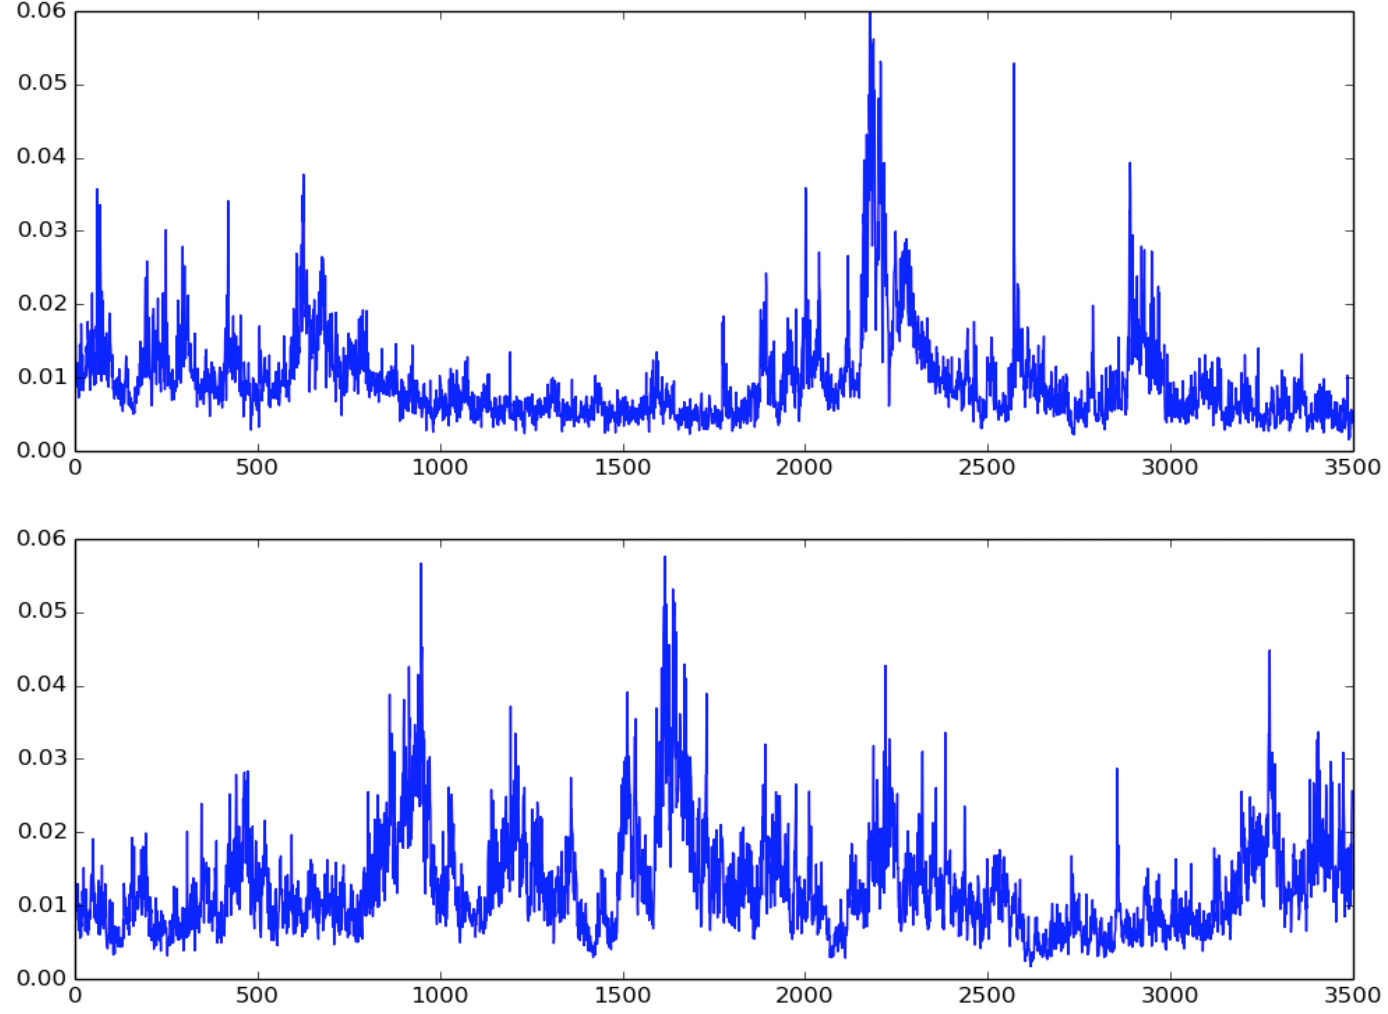
\includegraphics[width=0.85\textwidth ]{figs/gatheral_2014_fig36_p22}
    \caption{Extracted directly from Gatheral et al., 2014, \cite[Figure~3.6]{gatheral2014volatility}. Sample path of the model generated volatility (bottom) compared with the S\&P volatility (top). The x-axis represents the time to maturity in days, and the y-axis represents volatility.}
    \label{fig:gatheral_2014_volplots}
\end{figure}

As is highlighted in \cite{gatheral2014volatility}, we see a striking similarity between both plots of Figure \ref{fig:gatheral_2014_volplots}, with both exhibiting periods of high volatility, followed or preceded by periods of low volatility.  Recall that choosing $H<1/2$ means that the increments of the fractional Brownian motion are negatively correlated. In this analysis, $H$ was chosen to be less than 1/2 which would capture this certain trend in the model, as was discussed in Section \ref{sec:fractionalBm}. The smoothness of the volatility process could be captured through this model by tuning $H$.

It is important to mention that RFSV model is not long memory. However, when applying standard statistical estimators to data simulated by the RFSV model, long memory was incorrectly found to be present, with parameters estimated similar to those found in other studies. This led Gatherall et al. to conclude that this is why volatility having a long memory property is often accepted as a stylized fact. 

A more recent paper \cite{fukasawa2020volatility} also showed that volatility has to be rough through an arbitrage argument involving the power law associated with implied volatility which is empirically observed in option markets \cite{Carr2001}. The power law of implied volatility, also known as the 'volatility smirk', aims to approximate the implied volatility curve of some options, which have a higher implied volatility for low strikes and a lower implied volatility for higher strikes. This shape is shown to be a negative skew, where the curve is steep for low strikes and flattens out for higher strikes (hence the name 'volatility smirk'). Fukusawa showed in \cite{fukasawa2020volatility} that there is an arbitrage opportunity if volatility isn't rough given an option market obeying the power law given in Equation \ref{eqn:powerlaw}.

\begin{equation}
\label{eqn:powerlaw}
\frac{\sigma_{BS}(K,T) - \sigma_{BS}(K',T)}{K-K'}\propto T^{H-1/2}
\end{equation}

where $K \approx 0$, $K' \approx 0$, with $H \approx 0$ when $T \approx 0$. Here, $\sigma_{BS}(K,T)$ is the Black-Scholes implied volatility with log strike $K$ and time to maturity T. This arbitrage opportunity is under the assumption that the asset price is a positive continuous It\^o semimartingale. 

Even more recent studies such as \cite{jusselin2018noarbitrage} have explored the origin of rough volatility whereby it was proved that rough volatility is a consequence of the no arbitrage principle and market impact. In this context, market impact is defined to be the fact that on average for a given asset, a buy order increases it's price and a sell order causes a decrease in it's price. Given the astounding evidence discovered through such studies, it has been thoroughly accepted as a stylized fact that volatility is indeed rough. 

\subsection{Pricing with rough volatility}

In this section, we are going to describe how the Rough Fractional Stochastic Volatility model can be used to price contingent claims and thus for option pricing. In particular, the Bergomi model is transformed into a Rough Bergomi Model, which has showed to fit the SPX volatility better than conventional Markovian stochastic models \cite{Bayer2016pricing}. 
\\

As stated in the previous section,  distributions of increments of the logarithm of realized variance were found to be close to Gaussian and the time series of the realized variance was found to be described by the model:

\begin{equation}
\label{eq:realizedvariance}
    log\sigma_{t+\Delta} - log\sigma_{t} = \nu (W_{T+\Delta}^{H} - W_{t}^{H})
\end{equation}

where $W^{H}$ is a fBM, which is just the RFSV model with $\alpha = 0$.

Now, let consider the Mandelbort-Van Ness representation of fBM $W_{H}$:

$$W_{t}^{H} = C_{H} [\int_{-\infty}^{t} \frac{dW_{s}^{P}}{(t-s)^{\gamma}} - \int_{-\infty}^{0} \frac{dW_{s}^{P}}{(-s)^{\gamma}}]$$


If we substitute the previous equation into \ref{eq:realizedvariance},then the evolution of the instantaneous variance $\nu_{u}$ under the physical measure P would be:
\begin{equation}
\label{eq:realizedvariance}
    log\upsilon_{u} - log\upsilon_{t} := 2  \nu [M_{t}(u) + Z_{t}(u)]
\end{equation}

Let introduce 



Stochastic models such as Hull and White, Heston, and SABR are criticized for generating implied volatility surfaces, which shapes differ substantially from that ones observed empirically in the market. In fact, a relevant characteristic that may distinguish from different volatility models is the way to approach the term structure of at-the-money (ATM) volatility skew, defined as:

\begin{equation}
    \lvert \frac{\partial}{\partial k} \sigma_{BS}(k,\tau) \rvert_{k = 0}
\end{equation}

, where $\tau = T - t$ is the time to maturity, and $k$ is the log-moneyness equal to $log(\frac{K}{S_{t}})$. Stochastic models present the ATM volatility skew to be constant for short dates and inversely proportional to $\tau$ for long dates. In fact, evidence has showed that skew volatility is proportional to $\tau^{-\alpha}$, for $0<\alpha<1/2$. 

\begin{figure}[htpb]
    \centering
    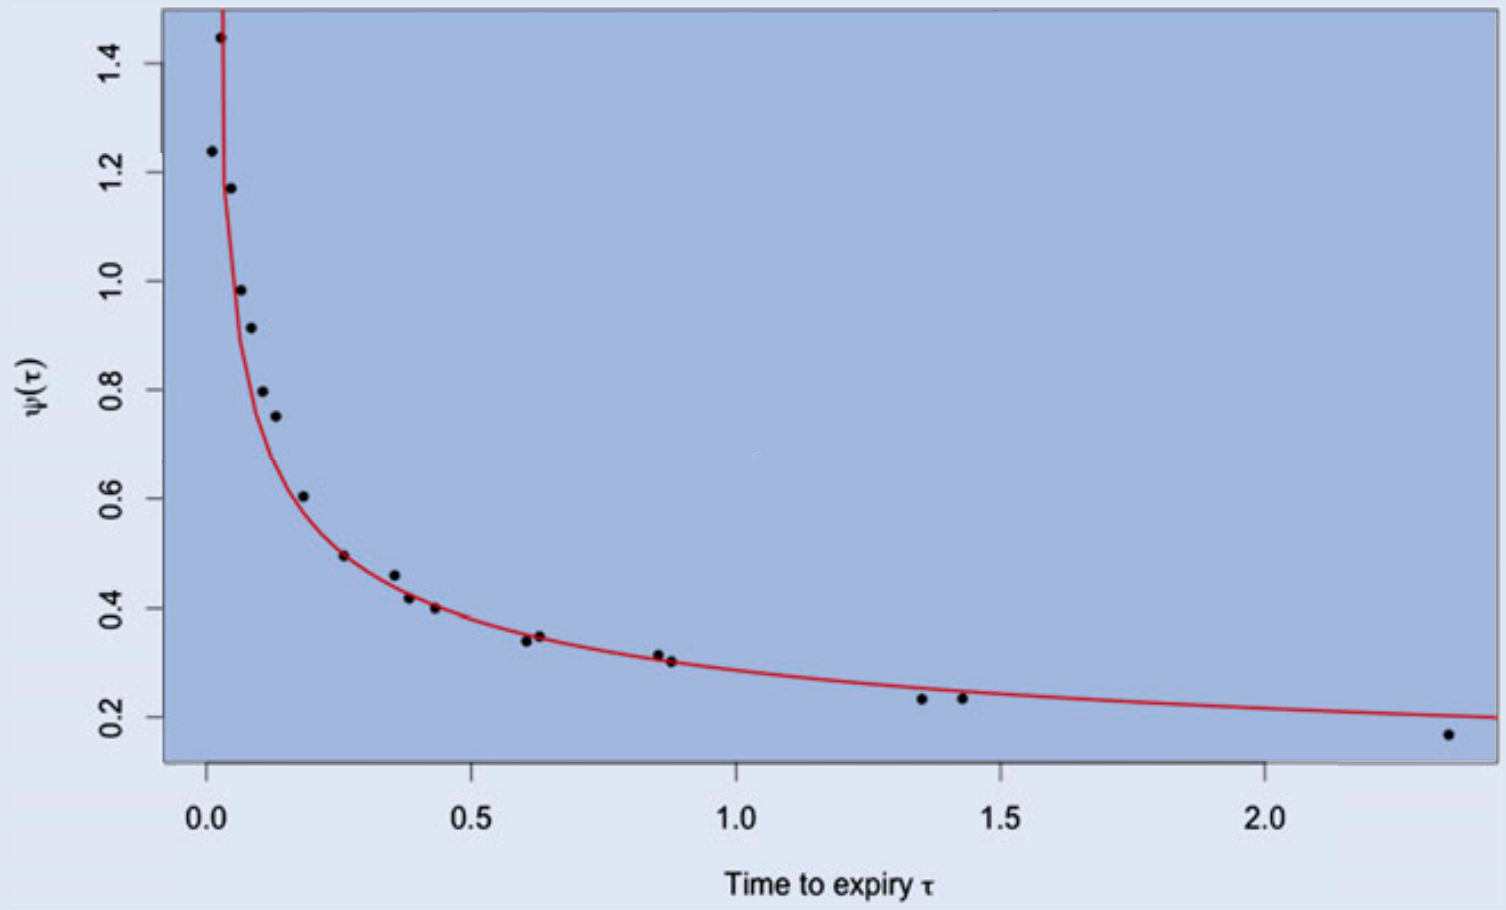
\includegraphics[width=0.85\textwidth ]{figs/Bayer2016_fig2.png}
    \caption{Extracted from Bayer et al., 2016  \cite[Figure~2]{Bayer2016pricing}. Plot shows change in volatility skew $\psi(\tau)$ with respect to $\tau$, time to expiry. The points are non-parametric estimates of the S&P at-the-money volatility skews as of 14/08/13. Red curve is the power-law fit $\psi(\tau) = A\tau^{−0.407}$, where $\tau$ is measured in years.}
    \label{fig:gatheral_2014_volplots}
\end{figure}

Bergomi and Guyon (2012) derive a small noise expansion for the smile in a stochastic volatility model making use of a forward variance curve, defined as the expectation under the pricing measure of the future instantaneous variance. In this way, given a stochastic model written in the forward curve form, it can be computed the term structure of ATM skew. The n-factor Bergomi variance curve model can be written as:

\begin{equation}
\label{eq:Bergomimodel}
    \xi_{t}(u) = \xi_{0}(u) \epsilon(\sum_{i=1}^{n} \eta_{i} \int_{0}^{t} e^{-K_{i}(u-s) dW_{s}^(i)}))
\end{equation}

where $\eta_{.}$ denotes the stochastic exponential. In this case, the Bergomi model generates a term structure volatility skew of the form:

$$\sum_{i=1}^{} \frac{\eta_{i}}{K_{i}} (1- \frac{1-e^{-K_{i}} \tau}{{K_{i}} \tau})$$

Thus, to generate the empirically observed form of $\tau^{-\alpha}$ for some $\alpha$ to replace the exponential kernels in \ref{eq:Bergomimodel} with a power-law kernel.

\subsection{The Rough Heston volatility Model}
\label{sebsec:rough_heston}
The classical Heston model has been introduced, as have the pitfalls  of these simplistic early option pricing models. The Classical Heston model does not agree with time series in practise, and does not generate a volatility surface similar to that observed, however there are benefits to the various parameters which make the model tractable, and when applying a rough volatility framework. Small Hurst parameters & fBM are introduced and the Ricatti characteristic function can be replaced with with a fractional Ricatti characteristic function to form the rough Heston model to produce behaviour seen in both historical & implied volatility, this has been well discussed in \cite{OElEuch2018} and \cite{ElEuchRosenbaum19}.

Before describing why Rough Heston models produce accurate implied volatility models, we must first introduce Hawkes process. A Hawkes process is a class of stochastic process, pleasantly articulated in \cite{laub2015hawkes}, which has a "self-exciting" characteristic, whereby each time step, or "arrival" over time, within a process leads to excitement which gives a greater probability of exaggerating the characteristics of the process experienced at current time step in the subsequent time step. When a Hawkes process is interpreted as a model of a trad-able asset price over time, it is clear to see how this can be successfully applied to the fickle behaviors of financial market, where large volumes of sales/buying of an asset leads to further selling/buying, and the resulting sensational decrease/increase of the asset price. This behaviour is most famously seen in large financial crashes (the 2008 financial crisis, Brexit, flash crash of 2010), or short term economic bubbles, and can be seen in Figure \ref{fig:gatheral_2014_volplots}. 

By sequencing a large number of Hawkes type point processes in \cite{omar2016microstructural}, it was found that these converge to a Rough Heston Model over long run result with careful construction considerations. Micro-structures of the Rough Heston were creating via  ultra-high-frequency Hawkes style price models sequences with the following stylized facts of the modern markets: 
\begin{enumerate} 
\item The majority of orders in the market are reactive algorithmic trades with no true economic rationale (described as highly endogenous). 
\item Arbitrage scenarios are highly unlikely due to the high frequency nature of the orders made in the market.  
\item Large algorithmic transactions, split over time and not in one order,  make up a large proportion of transactions in the market.
\item There is bid-ask asymmetry: meaning the markets shall react differently to a market maker selling an asset as opposed to buying. The price in the market of a given asset shall likely increase when a market maker buys this asset, however the change in the assets market price is likely to be of greater (negatively) upon a market maker selling this asset. This is a result of the availability of this asset in the market reduces upon a buying, but increases when sold. 
\end{enumerate}

Prior to defining the Rough Heston model we must return to the fBM, $(\textit{$W^H_t$})$, with Hurst parameters $\textit{H} \in (0,1)$ to be represented in the Mandelbrot-Van Ness representation:

\begin{equation}
\label{eqn:MvN_Hurst}
{W^H_t} = \frac{1}{\Gamma(H + \frac{1}{2})} \int_{0}^{-\infty} ((t-s)^{H-\frac{1}{2}} - (-s)^{H - \frac{1}{2}})W^H_s + \frac{1}{\Gamma(H + \frac{1}{2})} \int_{0}^{-\infty} (t-s)^{H-\frac{1}{2}}W^H_s
\end{equation}
We can see how influential  the kernel  $(t-s)^{H-\frac{1}{2}}$ is within rough volatility dynamics when $H<\frac{1}{2}$, and that the process: 
$$\int_{0}^{-\infty} (t-s)^{H-\frac{1}{2}} dW^s$$
has Holder regularity for $H - \epsilon$, for any $\epsilon>0$. El Euch et al.incorporated this kernel, $(t-s)^{\alpha-1}$, to the classical Heston model to introduce a rough volatility-type model, defining the rough Heston Model.

\begin{equation}
\label{eqn:rough_heston}
v_t = v_0 + \frac{1}{\Gamma(\alpha)} \int_{0}^{t} (t-s)^{\alpha-1} \kappa (\theta - v_s)ds + \frac{1}{\Gamma(\alpha)} \int_{0}^{t} \xi\sqrt{v_s}dW_s^{v}
\end{equation}

Where $\alpha = H+\frac{1}{2}$ and $\kappa, \theta, v_0$ and $\xi$ are all positive and equivalent to Equation \ref{eqn:classic_heston_var}. $\rho$ continues to be the correlation of $dW^S_t$ and $dW^v_t$. This model was found to be well defined when ${\alpha} \in (\frac{1}{2},1)$ the volatility trajectories almost surely have Holder regularity $\alpha - \frac{1}{2} -\epsilon$, as for Equation \ref{eqn:MvN_Hurst}, where for any $\epsilon>0$. It is important to note that when $\alpha$ = 1 we achieve the classical Heston Model. 

To continue with a selected Hurst parameter of $H < \frac{1}{2}$ a la \cite{gatheral2014volatility}. The Rough Heston model will be non-Markovian and $v_t$ is no longer a semi-martingale. This provides perfect motivation for El Euch et al., to design micro-structures of Hawkes point processes to model the "nearly unstable" behaviour of past events, and go on to demonstrate that combining the convergence results of these processes yield the characteristic function of the log-price of the rough Heston model. The suitability of these results can be seen in Figure \ref{fig:elEuch_1}. \emph{Finlay - why do these results show suitability??? What feature is it about these graphs that shows it? Do we need all four?}

\begin{figure}[htpb]
    \centering
    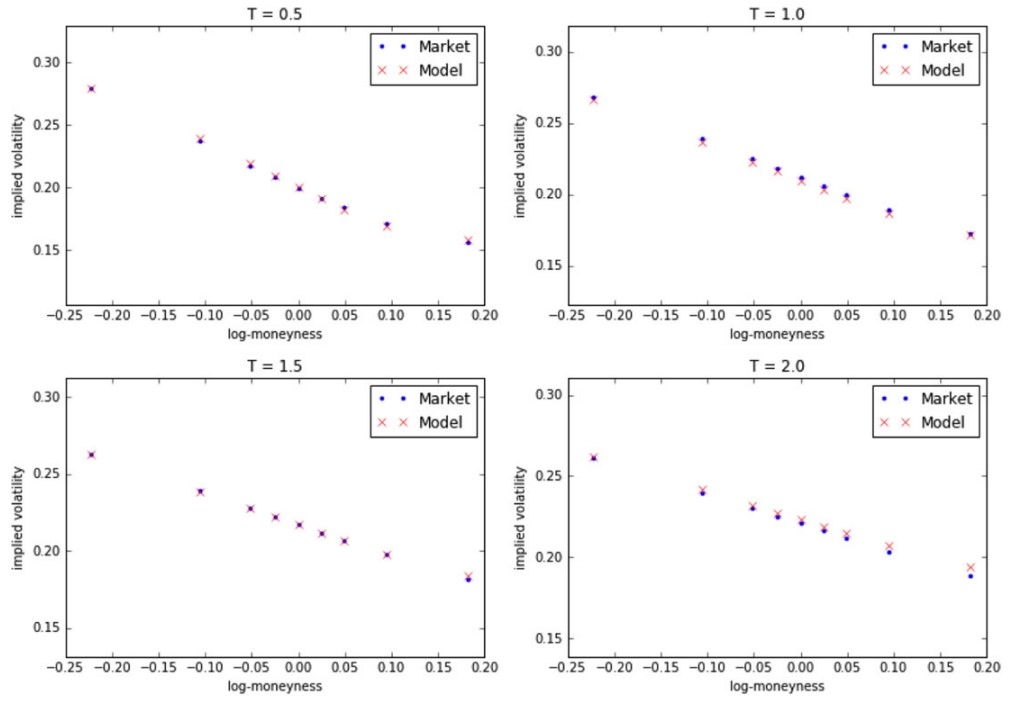
\includegraphics[width=0.85\textwidth ]{figs/elEuch_1.jpg}
    \caption{Extracted directly from El Euch and Rosenbaum, 2016, \cite[Figure~5.1]{omar2016microstructural}. Implied volatility surface calibration with a rough Heston model.}
    \label{fig:elEuch_1}
\end{figure}

One additional note on the suitability of the rough Heston model is that the  "self-exciting" characteristics which the Hawkes micro-processes which jump in probability based on past events negates considerations of introducing any "jump processes", which are generally discouraged in modern models. 

\section{Computational Advancements in Pricing with Rough Volatility Models}
\label{sec:comp_advancement}

Moving to a generalised setting, we now focus on rough volatility models in general that we know are driven by fBM. As mentioned in \cite{jacquier2020deep}, the use of fBM in such models carries a computational burden with it. In terms of option pricing, this restricts the use of several pricing tools such as the Black-Scholes formula and other pricing PDE's due to the non-deterministic nature of the volatility process.  Pricing via Monte Carlo simulation of the asset price and volatility processes is perhaps the one pricing tool that works but it can be slow in approximating continuous time solutions within a sufficient level of accuracy, especially for simulating non-Markovian process due to the extra memory required to store previous process states. Here, we give a brief overview of some theories that were introduced to combat the computational expense of exact Monte Carlo simulation of the volatility process. Namely, we discuss the Hybrid scheme in \cite{Bennedsen_2017}, the Markovian representation of fBM in \cite{harms2020strong} and the extension of the Donsker theorem to fBM in \cite{horvath2019functional}. These methods were introduced to improve the efficiency of the simulation of fBM and rough volatility processes while maintaining a reasonable level of accuracy.

\subsection{The Hybrid Scheme}
\label{subsec:hybrid_scheme}
The Hybrid Scheme was introduced in \cite{Bennedsen_2017} in which they study simulation methods for Brownian semistationary processes. A Brownian semistationary process is given by Equation \ref{eqn:semistationary}. 

\begin{equation}
\label{eqn:semistationary}
X(t)=\int_{-\infty}^t g(t-s) \sigma(s) dW(s),  \ \  t\in\mathbb{R}
\end{equation}

where $\sigma$ is a predictable process with respect to the given filtration. It is mentioned in \cite{Bennedsen_2017} that when $g(x) \propto x^\alpha$ and $\alpha \in (-\frac{1}{2}, \frac{1}{2}) \setminus \{0\}$, the process behaves (locally) like a fBM with Hurst parameter $H=\alpha+1/2$.  Therefore, being able to efficiently simulate such a process would help to improve computational efficiency for pricing in some rough volatility models.  

The Hybrid scheme involves approximating the function $g$ using a step function except for near 0, where a power function is used for approximation. Through a series of derivations, the resulting discretisation scheme is written as a linear combination of a Riemann sum and Wiener integrals. The scheme is given by Equation
\ref{eqn:hybrid}.  

\begin{equation}
\label{eqn:hybrid}
X_n(t) = \hat{X}_n(t) + \tilde{X}_n(t)
\end{equation}

where

\begin{equation}
\hat{X}_n(t) = \sum_{k=1}^{\kappa} L_g(\frac{k}{n}) \sigma (t-\frac{k}{n}) \int_{t-\frac{k}{n}}^{t-\frac{k}{n}+\frac{1}{n}}(t-s)^\alpha dW(s),
\end{equation}

and

\begin{equation}
\tilde{X}_n(t)=\sum_{k=\kappa+1}^{N_n}g(\frac{b_k}{n})\sigma(t-\frac{k}{n})(W(t-\frac{k}{n}+\frac{1}{n})-W(t-\frac{k}{n})),
\end{equation}

with $L_g$ chosen so that

\begin{equation}
g(t-s) \approx (t-s)^\alpha L_g(\frac{k}{n}), \ \ t-s \in [\frac{k-1}{n},\frac{k}{n}]
\end{equation}

In terms of applying the scheme to rough volatility models, the Hybrid Scheme was used for option pricing in the Bergomi model via Monte Carlo simulation, as is discussed in the referenced paper. Using the Hybrid Scheme in this setting simplified the simulation process (see page 20 of \cite{Bennedsen_2017}) and reduced the computational cost compared to producing exact simulations from the model. The results from using the scheme were then compared to exact results from the Bergomi model and it showed that the Hybrid Scheme was able to produce almost exactly the same volatility smile as that produced by exact simulation from the Bergomi model while being significantly more efficient.

\subsection{Markovian Representation of fBM}
\label{subsec:markovian_rep_fBm}
Without going into too much detail, it was shown in \cite{harms2020strong} that fBM can be approximated by a Markovian representation consisting of the sum of $n$ weighted Orstein-Uhlenbeck processes.  Based on a set of assumptions outlined in the paper, the approximation is given by Equation \ref{eqn:markov_approx}.

\begin{equation}
\label{eqn:markov_approx}
W_t^{H,n} = \sum_{i=1}^n w_{n,i} \int_0^t e^{-(t-s)x_{n,i}}dW_s, \ \ t \in [0,T] 
\end{equation}

where the $x_{n,i}$ are so-called 'speeds of mean reversion' and the $w_{n,i}$ are weights, with both terms taking positive values. This approximation forms part of a theorem which states that fBM is approximated by this representation at a rate of $n^{-r}$ for any given $r>0$.  This theorem also states that under this approximation, put prices in the Bergomi model also converge at a rate of $n^{-r}$. 

Using this approximation for fBM, a discrete Monte Carlo scheme for the rough Bergomi model can be acheived and since the representation is Markovian, it improves efficiency. It is also mentioned that in terms of error and complexity,  this method outperforms several other computational methods. However, it is outperformed by the Hybrid Scheme that was discussed earlier. 

\subsection{Extension of Donkser's Theorem to fBM}
Like the previous examples, the motivation of extending Donsker's theorem for Brownian motion to fBM is to be able to approximate fBM in a way that would reduce computational cost. To give some context,  we state Donsker's Theorem.

 \textbf{Theorem (Donsker)}: \emph{Let} $\epsilon_1,...,\epsilon_n$ \emph{be i.i.d. random variables with mean 0 and variance} $\sigma^2$. \emph{Then for} $X^{(n)}$ defined by
 
 \begin{equation}
 \label{eq:donsker_thm}
 X_t^{(n)} = \frac{1}{\sigma \sqrt{n}} (S_{\lfloor nt \rfloor} - (nt - \lfloor nt \rfloor) \epsilon_{\lfloor nt \rfloor + 1}), \ \ t\in[0,1]
 \end{equation}
 
 where,
 
\begin{equation}
S_m = \sum_{i=1}^i \epsilon_m
\end{equation}

then $X_t^{(n)} \rightarrow W_t$ \emph{in distribution for} $t\ge0$ \emph{on the space of continuous functions, where} $W_t$ \emph{is classical Brownian motion}.

By being able to extend this theorem to fBM, one could approximate it using i.i.d. sequences of random variables leading to a simplified simulation process. Again, without going into too much detail, an extension of this theorem was proved in \cite{horvath2019functional} which approximates the logarithm of the stock price under a rough volatility model under the assumption that the i.i.d. random variables have a finite second moment (variance in this case) and a number of other conditions which we will omit but can be found in the paper. In terms of pricing, this approximation could then be applied to fractional binomial trees, which opens the door to pricing American-type options under rough volatility models. However, the branches of such trees generally do not recombine which adds to the complexity of this pricing method.   

\section{Conclusion}
\label{sec:conclusion}
 

\emph{Our main result is
that log-volatility behaves essentially as a fractional Brownian motion
with Hurst exponent H of order 0.1, at any reasonable time scale.
This leads us to adopt the fractional stochastic volatility (FSV) model
of Comte and Renault [16]. We call our model Rough FSV (RFSV)
to underline that, in contrast to FSV, H < 1/2.}

Long memory volatility referred to the slow decay of the autocorrelation function.

In the vast majority of papers this section is not present. It could be used to provide a brief summary of the paper or some areas for further research. Most likely it won't be useful for the final essays.

The final point in this document is of high importance. 

\bibliographystyle{unsrt}
%  \bibliographystyle{plain}  % Or use the `amsrefs' package (http://www.ams.org/tex/amsrefs.html)!
\bibliography{my_bibtex_file.bib}
 \addcontentsline{toc}{section}{Bibliography}
\end{document}
